\chapter{Introduction to Spatial Econometric}\label{chapater:Introduction}


%===============================================================
\section{Why do We Need Spatial Econometric?}\label{sec:why_se}
%===============================================================

An essential consideration in any study involving spatial units, such as cities, regions, or countries, is the potential relationships and interactions between them. For instance, when modeling pollution at the regional level, it becomes impractical to treat each region as an independent entity. Regions cannot be analyzed in isolation since they are spatially interrelated through ecological and economic interactions.

Consider Figure \ref{fig:example_poll}, where Region 3 (R3) is highly industrialized, while Regions 1, 2, 4, and 5 are residential areas. If Region 3 increases its economic activity, pollution will not only rise within that region but will also affect neighboring regions. It is anticipated that contamination will increase in Regions 1 and 5, albeit to a lesser extent. These spatial externalities from R3 can be generated by both spatial-economic interactions (e.g., transportation of inputs and outputs from Region 3) and spatial-ecological interactions (e.g., carbon emissions).

%-------------------------------------------
\begin{figure}[h]
\caption{Environmental Externalities}
\label{fig:example_poll}
\centering
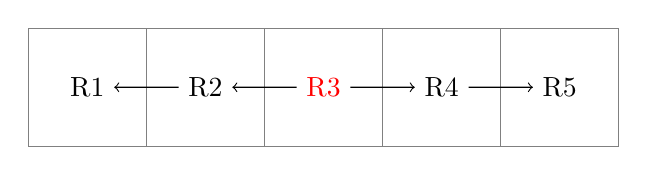
\begin{tikzpicture}[scale = 1.5]
\draw[color = gray] (0,0) grid[xstep = 1cm, ystep = 1cm] (5,1);
\node (R1) at (.5, .5) {R1};
\node (R2) at (1.5,.5) {R2};
\node (R3) [color =  red]  at (2.5,.5) {R3};
\node (R4) at (3.5,.5) {R4};
\node (R5) at (4.5,.5) {R5};
\draw [->] (R3) -- (R2);
\draw [->] (R3) -- (R4);
\draw [->] (R2) -- (R1);
\draw [->] (R4) -- (R5);
\end{tikzpicture}
\end{figure}
%-------------------------------------------

Similarly, when studying crime at the city level, it is crucial to incorporate the possibility that crime is localized. The identification of concentrations or clusters of higher criminal activity has become a central mechanism for targeting criminal justice and crime prevention responses. These crime clusters, commonly referred to as \textbf{hotspots}, represent geographic locations with high crime concentrations relative to the overall distribution of crime across the entire region of interest.

Both examples implicitly highlight the significance of geographic location and distance. They underscore the importance of the first law of geography, as articulated by Waldo Tobler: \emph{``everything is related to everything else, but near things are more related than distant things''}. This foundational principle gives rise to fundamental concepts such as \textbf{spatial dependence} and \textbf{spatial autocorrelation}.\index{Tobler's law}

%---------------------------------------------
\subsection{Spatial Dependence}\label{sec:spatial_dependence}\index{Spatial dependence}
%---------------------------------------------

Spatial dependence occurs when the values observed at one location or region, say observation $i$, depend on the values of neighboring observations at nearby locations. Formally, we can express this as:
\begin{equation*}
  y_i = f(y_j),\quad i = 1,\ldots,n\;, j\neq i.
\end{equation*}

In simpler terms, what happens in region $i$ depends on what happens in region $j$ for all $j \neq i$. For example, using our previous example displayed in Figure \ref{fig:example_poll}, we would like to estimate 
\begin{equation*}
  \begin{aligned}
y_1 & = \beta_{21} y_2 + \beta_{31} y_3 + \beta_{41} y_4 + \beta_{51} y_5 + \epsilon_1, \\
y_2 & = \beta_{12} y_1 + \beta_{32} y_3 + \beta_{42} y_4 + \beta_{52} y_5 + \epsilon_2, \\
y_3 & = \beta_{13} y_1 + \beta_{23} y_2 + \beta_{43} y_4 + \beta_{53} y_5 + \epsilon_3, \\
y_4 & = \beta_{14} y_1 + \beta_{24} y_2 + \beta_{34} y_3 + \beta_{54} y_5 + \epsilon_4, \\
y_5 & = \beta_{15} y_1 + \beta_{25} y_2 + \beta_{35} y_3 + \beta_{45} y_5 + \epsilon_5, 
\end{aligned}
\end{equation*}
%
where $\beta_{ji}$ represents the effect of pollution in region $j$ on region $i$. However, this model becomes impractical as it would result in a system with many more parameters than observations. With $n = 5$ observations, we would have to estimate 20 parameters, exceeding the available degrees of freedom. Intuitively, allowing for dependence relations between a set of $n$ observations/locations introduces potentially $n^2 - n$ relations, accounting for the exclusion of dependence on oneself.

The crucial point is that, under standard econometric modeling, incorporating spatial dependency in such a manner is impractical. However, as we will explore in the next sections, we can efficiently integrate spatial relationships using the so-called \textbf{spatial weight matrix}. 

%===========================================
\subsection{Spatial Autocorrelation}\label{sec:Spatial_autocorrelation}
%===========================================

Another crucial concept is \textbf{spatial autocorrelation}\index{Spatial autocorrelation}. In a spatial context, autocorrelation denotes the correlation between the values of a variable at two different locations. It can also be defined as the correlation between the same attribute at two (or more) different locations or the coincidence of values' similarity with location similarity. Essentially, spatial autocorrelation investigates whether the presence of a variable in one region of a spatial system makes the presence of that variable in neighboring regions more or less likely.

The counterpart of spatial autocorrelation (and spatial dependency) is spatial randomness. Spatial randomness implies the absence of any discernible spatial pattern in the data. In other words, the value observed in one spatial unit is equally likely as in any other spatial unit. Spatial randomness is important because it will form the null hypothesis later. If rejected, there is evidence of spatial structure.

As an illustrative example, Figure \ref{fig:MR} depicts the spatial distribution of poverty in the communes of the Metropolitan Region, Chile. It reveals a discernible spatial pattern where communes with similar poverty rates are clustered.
\begin{figure}[ht]
  \caption{Spatial Distribution of Poverty in Metropolitan Region, Chile}
    \label{fig:MR}
    \centering
    	\begin{minipage}{.9\linewidth}
\begin{knitrout}
\definecolor{shadecolor}{rgb}{0.969, 0.969, 0.969}\color{fgcolor}

{\centering \includegraphics[width=8cm,height=8cm]{figure/MetroRegion-1} 

}


\end{knitrout}
\footnotesize
		\emph{Notes:} This graph shows the spatial distribution of poverty in the Metropolitan Region, Chile. 
	\end{minipage}	
\end{figure}

Formally, the presence of spatial autocorrelation can be expressed through the following moment conditions:
\begin{equation*}
  \cov(y_i, y_j) = \E(y_iy_j) - \E(y_i)\E(y_j) \neq 0 \;\; \text{for} \;\; i \neq j,
\end{equation*}
%
where $y_i$ and $y_j$ are observations on a random variable at locations $i$ and $j$ in space. Here, $i$ and $j$ can represent either points or areal units. Therefore, nonzero spatial autocorrelation exists between attributes of a feature defined at locations $i$ and $j$ if the covariance between feature attribute values at those points is nonzero. If this covariance is \textbf{positive} (i.e., if data with attribute values above the mean tend to be near other data with values above the mean), then we refer to it as \textbf{positive spatial autocorrelation}; conversely, if the opposite is true, we term it \textbf{negative spatial autocorrelation}. Figure \ref{fig:Autocorrelation} illustrates examples of positive and negative spatial autocorrelation.

\begin{figure}[ht]
  \caption{Spatial Autocorrelation}
    \label{fig:Autocorrelation}
    \centering
    	\begin{minipage}{1\linewidth}
\begin{knitrout}
\definecolor{shadecolor}{rgb}{0.969, 0.969, 0.969}\color{fgcolor}

{\centering \includegraphics[width=10cm,height=10cm]{figure/Autocorrelation-1} 

}


\end{knitrout}
\footnotesize
		\emph{Notes:} Spatial Autocorrelation among 400 spatial units arranged in an 20-by-20 regular square lattice grid. Different gray-tones refer to different values of the variable ranging from low values (white) to high values (black). The left plot shows positive spatial autocorrelation, whereas right plot shows negative spatial autocorrelation. 
	\end{minipage}	
\end{figure}

Positive autocorrelation is more commonly observed, but negative autocorrelation does exist. Instances of negative autocorrelation can be found in studies on welfare competition or federal grants competitions among local governments \citep{saavedra2000model, boarnet2002federal}, regional employment \citep{filiztekin2009regional, pavlyuk2011spatial}, cross-border lottery shopping \citep{garrett2002revenue}, foreign direct investment in OECD countries \citep{garretsen2009fdi}, and the locations of the Turkish manufacturing industry \citep{basdas2009spatial}. In essence, our interest lies in studying non-random spatial patterns and explaining this non-randomness. Potential causes of non-randomness, as outlined by \cite{gibbons2015spatial}, include:

\begin{enumerate}
    \item Economic agents may be randomly allocated across space, but some characteristics of locations vary across space and influence outcomes.
    \item Location may have no causal effect on outcomes, but outcomes may be correlated across space because heterogeneous individuals or firms are non-randomly allocated across space.
    \item Individuals or firms may be randomly allocated across space, but they interact in a way that decisions by one agent affect the outcomes of other agents.
    \item Individuals or firms may be non-randomly allocated across space, and the characteristics of others nearby directly influence individual outcomes.
\end{enumerate}

%********************************
\section{Spatial Weight Matrix}\index{Weight matrix}
%********************************

One of the crucial issues in spatial econometric is the problem of formally incorporating spatial dependence into the model. As we reviewed in Section~\ref{sec:spatial_dependence}, the main problem is that we have more parameter than observations. So, the question is: What would be a good criteria to define closeness in space? Or, in other words, how to determine which other units in the system influence the one under consideration?

The device typically used in spatial analysis to define the concept of closeness in space is the so-called ``spatial weight matrix'', or more simply, $\mW$ matrix. Assuming there are $n$ spatial objects (regions, cities, countries), the $\mW$ matrix is a square matrix of dimension $n \times n$. This matrix imposes a structure in terms of identifying neighbors for each location, assigning weights that measure the intensity of the relationship among pairs of spatial units. Each element $(i,j)$ of $\mW$, denoted as $w_{ij}$, expresses the degree of spatial proximity between the pair. The matrix can be represented as follows:
\begin{equation*}
\mW = \begin{pmatrix}
        w_{11} & w_{12} & \hdots & w_{1n} \\ 
        w_{21} & w_{22} & \hdots & w_{2n} \\
        \vdots & \vdots & \ddots & \vdots \\
        w_{n1} & w_{n2} & \hdots & w_{nn} 
      \end{pmatrix}.
\end{equation*}

Generally, we assume that the diagonal elements of this ``spatial neighbors'' matrix are set to zero, indicating that ``regions are not neighbors to themselves''.

A more formal definition of a spatial weight matrix is as follows:

%-----------------------------------------------------------------------------------
\begin{definition}[Spatial Weight Matrix]\index{Weight matrix!Definition}\label{def:W}
  Let $n$ be the number of spatial units. The spatial weight matrix, $\mW$, is a $n\times n$ \textbf{positive} and \textbf{non-stochastic} matrix with element $w_{ij}$ at location $i,j$. The values of $w_{ij}$ or the weights for each pair of locations are assigned by some preset rules which define the spatial relations among locations. By convention, $w_{ij} = 0$ for the diagonal elements.
\end{definition}
%-----------------------------------------------------------------------------------

Positive means that $w_{ij}\geq 0$ for all $i\neq j$. Thus, the interactions between spatial units cannot be negative. Non-stochastic means that the researcher takes $\mW$ as known \emph{a priori}, and therefore, all results are conditional upon the specification of $\mW$.

The definition of $\mW$ also requires a rule for $w_{ij}$. In other words, we need to figure out how to assign a real number to $w_{ij}$, for $i\neq j$, representing the strength of the spatial relationship between $i$ and $j$. There are several ways of doing that. But, in general, there are two basic criteria. The first type establishes a relationship based on shared borders or vertices of lattice or irregular polygon data (contiguity). The second type establishes a relationship based on the distance between locations. Generally speaking, contiguity is most appropriate for geographic data expressed as polygons (so-called areal units), whereas distance is suited for point data, although in practice, the distinction is not that absolute. 

%==========================================
\subsection{Weights Based on Boundaries}
%==========================================

Polygon or lattice data allow for the construction of contiguity-based spatial weight matrices, which represent spatial relationships among regions. A typical specification of the contiguity relationship in such matrices is given by:
\begin{equation*}
  w_{ij}= 
   \begin{cases}
      1 & \mbox{if $i$ and $j$ are contiguous,} \\ 
      0 & \mbox{if $i$ and $j$ are not contiguous.} 
   \end{cases}
\end{equation*}

In regular grids, the definition of contiguity can vary. Drawing an analogy to chess, three common contiguity criteria are rook contiguity, bishop contiguity, and queen contiguity. Each criterion defines neighborhood relationships differently, as detailed below.

\subsubsection{Rook Contiguity}\index{Weight matrix!Rook contiguity}

Rook contiguity considers two regions as neighbors if they share a common border or side. For example, in the regular grid shown in Figure~\ref{fig:Rook_cont_grid}, which contains 9 regions (each represented as a square), the neighbors of region 5 under the rook criterion are regions 2, 4, 6, and 8 (highlighted in red).

\begin{figure}[h]
\caption{Rook Contiguity}
\label{fig:Rook_cont_grid}
\centering
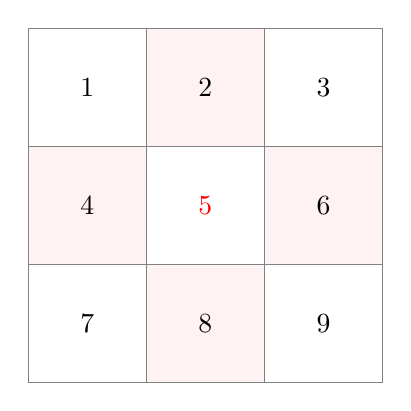
\begin{tikzpicture}[scale = 1.5]
\path [fill=red!5] (1,2) -- (2,2) -- (2,3) -- (1,3);
\path [fill=red!5] (1,0) -- (2,0) -- (2,1) -- (1,1);
\path [fill=red!5] (0,1) -- (1,1) -- (1,2) -- (0,2);
\path [fill=red!5] (2,1) -- (3,1) -- (3,2) -- (2,2);
\draw[color = gray] (0,0) grid[xstep = 1cm, ystep = 1cm] (3,3); % grid of 3 times 3
\node at (.5, 2.5) {1};
\node at (1.5, 2.5) {2};
\node at (2.5, 2.5) {3};
\node at (.5, 1.5) {4};
\node [color =  red] at (1.5,1.5) {5} ;
\node at (2.5,1.5) {6};
\node at (.5, .5) {7};
\node at (1.5,.5) {8};
\node at (2.5,.5) {9};
\end{tikzpicture}
\end{figure}

Using this criterion, the $9 \times 9$ spatial weight matrix $\mW$ is:
\begin{equation*}
  \mW = 
  \begin{pmatrix}
     0 & 1 & 0 & 1 & 0 & 0 & 0 & 0 & 0 \\
     1 & 0 & 1 & 0 & 1 & 0 & 0 & 0 & 0 \\
     0 & 1 & 0 & 0 & 0 & 1 & 0 & 0 & 0 \\
     1 & 0 & 0 & 0 & 1 & 0 & 1 & 0 & 0 \\
     0 & 1 & 0 & 1 & 0 & 1 & 0 & 1 & 0 \\
     0 & 0 & 1 & 0 & 1 & 0 & 0 & 0 & 1 \\
     0 & 0 & 0 & 1 & 0 & 0 & 0 & 1 & 0 \\
     0 & 0 & 0 & 0 & 1 & 0 & 1 & 0 & 1 \\
     0 & 0 & 0 & 0 & 0 & 1 & 0 & 1 & 0 \\
  \end{pmatrix}
\end{equation*}

\subsubsection{Bishop Contiguity}\index{Weight matrix!Bishop contiguity}

Under bishop contiguity, two regions are neighbors if they share a common corner. This criterion is less frequently used in practice. In Figure~\ref{fig:Bishop_cont_grid}, the neighbors of region 5 are regions 1, 3, 7, and 9 (highlighted in red). Note that regions located at the grid's interior have more neighbors than those along the periphery.

\begin{figure}[h]
\caption{Bishop Contiguity}
\label{fig:Bishop_cont_grid}
\centering
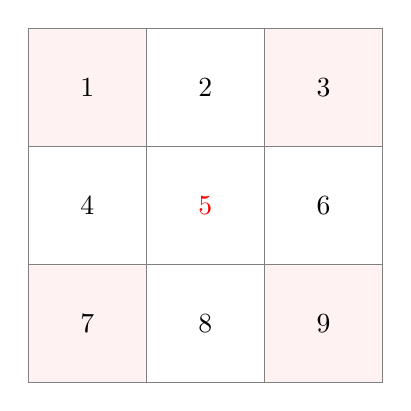
\begin{tikzpicture}[scale = 1.5]
\path [fill=red!5] (0,2) -- (1,2) -- (1,3) -- (0,3);
\path [fill=red!5] (0,0) -- (1,0) -- (1,1) -- (0,1);
\path [fill=red!5] (2,2) -- (3,2) -- (3,3) -- (2,3);
\path [fill=red!5] (2,0) -- (3,0) -- (3,1) -- (2,1);
\draw[color = gray] (0,0) grid[xstep = 1cm, ystep = 1cm] (3,3); % grid of 3 times 3
\node at (.5, 2.5) {1};
\node at (1.5, 2.5) {2};
\node at (2.5, 2.5) {3};
\node at (.5, 1.5) {4};
\node [color =  red] at (1.5,1.5) {5} ;
\node at (2.5,1.5) {6};
\node at (.5, .5) {7};
\node at (1.5,.5) {8};
\node at (2.5,.5) {9};
\end{tikzpicture}
\end{figure}

The corresponding $\mW$ matrix is:
\begin{equation*}
\mW = 
  \begin{pmatrix}
     0 & 0 & 0 & 0 & 1 & 0 & 0 & 0 & 0 \\
     0 & 0 & 0 & 1 & 0 & 1 & 0 & 0 & 0 \\
     0 & 0 & 0 & 0 & 1 & 0 & 0 & 0 & 0 \\
     0 & 1 & 0 & 0 & 0 & 0 & 0 & 1 & 0 \\
     1 & 0 & 1 & 0 & 0 & 0 & 1 & 0 & 1 \\
     0 & 1 & 0 & 0 & 0 & 0 & 0 & 1 & 0 \\
     0 & 0 & 0 & 0 & 1 & 0 & 0 & 0 & 0 \\
     0 & 0 & 0 & 1 & 0 & 1 & 0 & 0 & 0 \\
     0 & 0 & 0 & 0 & 1 & 0 & 0 & 0 & 0 \\
  \end{pmatrix}
\end{equation*}


\subsubsection{Queen Contiguity}\index{Weight matrix!Queen contiguity}

Queen contiguity considers two regions as neighbors if they share either a common side or a common corner. In Figure~\ref{fig:Queen_cont_grid}, the neighbors of region 5 include all surrounding regions: 1, 2, 3, 4, 6, 7, 8, and 9 (highlighted in red).

\begin{figure}[h]
\caption{Queen Contiguity}
\label{fig:Queen_cont_grid}
\centering
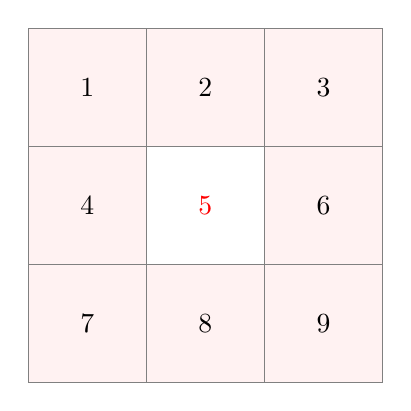
\begin{tikzpicture}[scale = 1.5]
\path [fill=red!5] (0,2) -- (1,2) -- (1,3) -- (0,3);
\path [fill=red!5] (0,0) -- (1,0) -- (1,1) -- (0,1);
\path [fill=red!5] (2,2) -- (3,2) -- (3,3) -- (2,3);
\path [fill=red!5] (2,0) -- (3,0) -- (3,1) -- (2,1);
\path [fill=red!5] (1,2) -- (2,2) -- (2,3) -- (1,3);
\path [fill=red!5] (1,0) -- (2,0) -- (2,1) -- (1,1);
\path [fill=red!5] (0,1) -- (1,1) -- (1,2) -- (0,2);
\path [fill=red!5] (2,1) -- (3,1) -- (3,2) -- (2,2);
\draw[color = gray] (0,0) grid[xstep = 1cm, ystep = 1cm] (3,3); % grid of 3 times 3
\node at (.5, 2.5) {1};
\node at (1.5, 2.5) {2};
\node at (2.5, 2.5) {3};
\node at (.5, 1.5) {4};
\node [color =  red] at (1.5,1.5) {5} ;
\node at (2.5,1.5) {6};
\node at (.5, .5) {7};
\node at (1.5,.5) {8};
\node at (2.5,.5) {9};
\end{tikzpicture}
\end{figure}


%=========================================
\subsection{Weights Based on Distance}\index{Weight matrix!Based on distance}
%=========================================

Weights can also be defined as a function of the distance between regions $i$ and $j$, denoted as $d_{ij}$. Typically, this distance is computed as the separation between centroids, although other significant points, such as capital cities or major urban centers, could also be used. Notably, unlike contiguity-based weights, distance-based matrices only require the coordinates of the relevant points.

Several methods exist to compute the distance between two spatial units. Let $x_i$ and $x_j$ represent the longitudes, and $y_i$ and $y_j$ denote the latitudes of regions $i$ and $j$. The \textbf{Minkowski}\index{Weight matrix!Minkowki} metric provides a general formula for distance:
\begin{equation*}
  d_{ij}^p = \left(\left|x_i - x_j\right|^p + \left|y_i - y_j\right|^p\right),
\end{equation*}
%
where $p$ is a parameter that allows flexibility in distance computation. A commonly used variant is the Euclidean distance, which corresponds to $p = 2$:
\begin{equation*}
  d_{ij}^e = \sqrt{(x_i - x_j)^2 + (y_i - y_j)^2}.
\end{equation*}

Another popular alternative is the Manhattan (or block) distance, which considers movement along east-west and north-south directions, i.e., along straight angles. This metric corresponds to $p = 1$:
\begin{equation*}
   d_{ij}^m = \left|x_i - x_j\right| + \left|y_i - y_j\right|.
\end{equation*}

While these metrics are suitable for treating the Earth as a plane, they may lack accuracy over larger distances due to the Earth's curvature. The Euclidean distance, for instance, represents the straight-line length on a map but might not align with the shortest path on the Earth's surface. For more accurate analyses, particularly for long-distance travel, the \textbf{great circle distance} is often preferred. This method considers the Earth's curvature and calculates the shortest path between two points on a sphere. The great circle distance is given by:
\begin{equation*}
d_{ij}^{cd} = r \times \arccos^{-1}\left[\cos|x_i - x_j| \cos y_i \cos y_j + \sin y_i \sin y_j \right],
\end{equation*}
%
where $r$ is the Earth's radius. The arc distance is obtained in miles with $r = 3959$ and in kilometers with $r = 6371$.

%=================================
\subsubsection{Inverse Distance}\label{sec:inverse_distance}
%=================================

Now, we must translate information about distances among spatial points into a weight scheme. The objective is to ensure that $w_{ij} \to 0$ as $d_{ij} \to \infty$. In simpler terms, as point $j$ gets farther from point $i$, the spatial weight $w_{ij}$ should decrease, aligning with Tobler's first law.

In the inverse distance weighting scheme, the weights are inversely proportional to the separation distance, as expressed by the following formula:
\begin{equation*}
  w_{ij} =
  \begin{cases}
  \frac{1}{d_{ij}^{\alpha}} & \mbox{if} \;\;i \neq j, \\
  0 & \mbox{if}\;\; i = j,
  \end{cases}
\end{equation*}
%
where the exponent $\alpha$ is a parameter that is usually set by the researcher. In practice, the parameters are seldom estimated, but typically set to $\alpha = 1$ or $\alpha = 2$. Consequently, the weights become the reciprocal of the distance: the greater the distance between spatial units, the smaller the spatial weight or connection. Conventionally, diagonal elements of spatial weights are set to zero to avoid division by zero in the case of inverse distance weights. Plugging in a value of $d_{ii} = 0$ would yield division by zero for inverse distance weights. 

\subsubsection{Negative Exponential Model}

In the negative exponential model, weights decrease exponentially with separation distance:
\begin{equation*}
  w_{ij} = \exp\left(-\frac{d_{ij}}{\alpha}\right),
\end{equation*}
%
where $\alpha$ is again a parameter that is commonly chosen by researcher. Since the weights are given by the exponential of the negative distance, the greater the distance between $i$ and $j$, the lower $w_{ij}$.

Both the inverse distance and negative exponential distance models rely on the parameter value, functional form, and the chosen distance metric. As the weights are inversely related to distance, larger distances yield smaller weights, and vice versa. A potential challenge arises when distances are so vast that inverse distance weights approach zero, possibly resulting in a spatial weight matrix with zero values. Additionally, issues may occur if the distance metric yields values less than one, which is typically undesirable \citep{anselin2014modern}. 

\subsubsection{$k$-nearest Neighbors}

An alternative approach to spatial weights that mitigates the issue of isolates involves selecting the $k$-nearest neighbors. Unlike the distance band, this relation is not symmetric. However, a challenge arises when ties occur—when multiple locations $j$ share the same distance from $i$. Several solutions exist to address ties, ranging from randomly selecting one of the $k$-th order neighbors to including all of them.

\subsubsection{Threshold Distance (Distance Band Weights)}

In contrast to the $k$-nearest neighbors method, the threshold distance specifies that a region $i$ is neighbor of $j$ if the distance between them is less than a specified maximum distance:
\begin{equation*}
  w_{ij}= 
   \begin{cases}
      1 & \mbox{if}\;\; 0\leq d_{ij} \leq d_{max}, \\ 
      0 & \mbox{if}\;\; d_{ij} > d_{max}.
   \end{cases}
\end{equation*}


To prevent isolates resulting from an excessively stringent critical distance, the distance must be chosen so that each location has at least one neighbor. Such a distance conforms to a max-min criterion, i.e., it is the largest of the nearest neighbor distances.

Importantly, a weights matrix derived from a distance band is always symmetric, as distance is inherently a symmetric relation.

%============================================
\subsection{Row-Standardized Weights Matrix}\index{Weight matrix!Row-standardization}
%============================================

In practical applications, spatial weights are rarely used in their raw binary (or distance) form. Instead, they are often transformed or standardized to improve interpretability and comparability. One common approach is to compute weighted averages, placing greater emphasis on nearby observations than on distant ones. To achieve this, a \textbf{row-standardized} weight matrix $\mW^s$ is defined, with elements $w_{ij}^s$ given by:
\begin{equation*}
w_{ij}^s = \frac{w_{ij}}{\sum_{j = 1}^n w_{ij}}.
\end{equation*}

This formulation ensures that all weights lie within the range of 0 to 1, facilitating the interpretation of matrix operations as an averaging of neighboring values. Moreover, row-standardization enhances the comparability of spatial parameters across models in various spatial stochastic processes \citep{AnselinBera1998}.

An additional feature of row-standardized matrices is that the sum of the weights in each row equals unity, and the total sum of all weights, $S_0 = \sum_i\sum_j w_{ij}$, equals the number of observations, $n$. This property simplifies the interpretation and application of the weights, as we will explore further in subsequent sections.

However, a key consequence of row-standardization is the loss of symmetry in the spatial weights matrix. While symmetric matrices have the desirable property of real eigenvalues, row-standardized matrices are generally asymmetric and do not preserve this characteristic. Nevertheless, row-standardization remains prevalent in applied work due to its intuitive interpretation and computational convenience.

Row-standardized matrices are also referred to as row-stochastic or Markov matrices. Formally, a row-stochastic matrix is defined as follows:
%%%%%%%%%%%%%%%%%%%%%%%%%%%%%%%%%%%%%%%%%%
\begin{definition}[Row-stochastic Matrix]
	A real $n\times n$ matrix $\mA$ is called \textbf{Markov} matrix or \textbf{row-stochastic matrix} if 
		\begin{enumerate}
			\item $a_{ij} \geq 0$ for $1\leq i, j \leq n$;
			\item $\sum_{j=1}^n a_{ij} = 1$ for $1\leq i \leq n$
		\end{enumerate}
\end{definition}
%%%%%%%%%%%%%%%%%%%%%%%%%%%%%%%%%%%%%%%%%%

An important property of row-stochastic matrices concerns their eigenvalues:

%%%%%%%%%%%%%%%%%%%%%%%%%%%%%%%%%%%%%%%%%%%
\begin{theorem}[Eigenvalues of row-stochastic Matrix]\label{teo:eigen_values}
	Every eigenvalue $\omega_i$ of a row-stochastic Matrix satisfies $\left|\vomega\right|\leq 1$
\end{theorem}
%%%%%%%%%%%%%%%%%%%%%%%%%%%%%%%%%%%%%%%%%%%

Therefore, the eigenvalues of the row-stochastic (i.e., row-normalized, row standardized or Markov) neighborhood matrix $\mW^s=(w_{ij}^s)$ are in the range $\left[-1, +1\right]$.

Finally, the behavior of $\mW^s$ is important for asymptotic properties of estimators and test statistics \citep[][pp. 244]{AnselinBera1998}. In particular, the $\mW$ matrix should be also exogenous, unless endogeneity is considered explicitly in the model specification. 

%============================================
\subsection{Spatial Lagged Variables}\label{sec:spatial_lag_var}\index{Weight matrix!Spatial lag}
%============================================

Having explored the spatial weight matrix, we can now introduce the concept of  \textbf{spatially lagged variables} or \textbf{spatial lag operator}. The spatial lag operator takes the form $\vy_L = \mW\vy$ with dimension $n \times 1$, where each element is given by $\vy_{Li} = \sum_{j = 1}^nw_{ij}y_j$, i.e., a weighted average of the $\vy$ values in the neighbor of $i$.

For example, consider 
\begin{equation*}
  \mW\vy =    \begin{pmatrix}
     0 & 1 & 0 \\
     1 & 0 & 1 \\
     0 & 1 & 0
  \end{pmatrix}
  \begin{pmatrix}
     10 \\
     50 \\
     30
  \end{pmatrix} =
  \begin{pmatrix}
     50 \\
     10 + 30 \\
     50
  \end{pmatrix}.
\end{equation*}

Using a row-standardized weight matrix:
\begin{equation*}
  \mW^s\vy =    \begin{pmatrix}
     0 & 1 & 0 \\
     0.5 & 0 & 0.5 \\
     0 & 1 & 0
  \end{pmatrix}
  \begin{pmatrix}
     10 \\
     50 \\
     30
  \end{pmatrix} =
  \begin{pmatrix}
     50 \\
     5 + 15 \\
     50
  \end{pmatrix}.
\end{equation*}

Consequently, for spatial unit $i$, the spatial lag of $y_i$, denoted a $\vy_{Li}$ (the variable $\mW\vy$ observed for location $i$) is:
\begin{equation*}
  \vy_{Li} = w_{i, 1}^sy_i + w_{i, 2}^sy_2 + \cdots + w_{i, n}^sy_n, 
\end{equation*}
%
or equivalently,
\begin{equation*}
  \vy_{Li} = \sum_{j = 1}^nw_{i,j}^sy_j,
\end{equation*}
%
where the weights $w_{ij}$ are the elements of the $i$th row of the matrix $\mW^s$ matched with the corresponding elements of the vector $\vy$. In other words, this represents a weighted sum of values observed at neighboring locations, excluding non-neighbors.

\begin{remark}
As stated by \citet[][p. 23-24]{anselin1988spatial}, standardization must be done with caution.\footnote{See also \citet[][p. 12]{elhorst2014spatial} and references therein.} For example, when the weights are based on an inverse distance function (or similar concept of distance decay), which has a meaningful economic interpretation, scaling the rows so that the weights sum to one may result in a loss of that interpretation. Can you give an example?
\end{remark}


%============================================
\subsection{Higher Order Spatial Weights}\label{sec:HSO}\index{Weight matrix!Higher order}
%============================================

To expand our understanding of geographical space as defined by the matrix $\mW$, we turn to the concept of higher-order neighbors. These are neighbors that are not directly adjacent but are reachable through other spatial units. For instance, we might consider the neighbors of a spatial unit's neighbors or even their neighbors' neighbors. To formalize this, we introduce the notion of \textbf{higher-order spatial weight matrices}.

The higher-order spatial weight matrix of order $l$, denoted as $\mW^l$, is defined as:
\begin{equation*}
  \mW^l = \underbrace{\mW \mW \cdots \mW}_{l \text{ times}}.
\end{equation*}

For example:
\begin{itemize}
\item The second-order spatial weight matrix is $\mW^2 = \mW\mW$.
\item The third-order spatial weight matrix is $\mW^3 = \mW \mW\mW$, and so on.
\end{itemize}

The element $w_{ij}$ in these higher-order matrices represents whether spatial unit $j$ is a neighbor of order $l$ to spatial unit $i$. Specifically:
\begin{itemize}
\item For $l = 2$, $w_{ij}$ equals 1 if $j$ is adjacent to a first-order neighbor of $i$, and 0 otherwise.
\item For $l = n$, $w_{ij}$ equals 1 if $j$ is adjacent to the $(n-1)$-order neighbors of $i$, and 0 otherwise.
\end{itemize}

To illustrate these points, consider the following spatial structure from example in Section \ref{sec:why_se}:
\begin{equation}\label{eq:W5x5}
\mW = \begin{pmatrix}
      0 & 1 & 0 & 0 & 0 \\
      1 & 0 & 1 & 0 & 0 \\
      0 & 1 & 0 & 1 & 0 \\
      0 & 0 & 1 & 0 & 1 \\
      0 & 0 & 0 & 1 & 0
      \end{pmatrix}.
\end{equation}

Then, $\mW^2 = \mW\mW$ based on the $5\times 5$ first-order contiguity matrix $\mW$ from \eqref{eq:W5x5} is:
\begin{equation}
\mW^2 = \begin{pmatrix}\label{eq:W25x5}
      1 & 0 & 1 & 0 & 0 \\
      0 & 2 & 0 & 1 & 0 \\
      1 & 0 & 2 & 0 & 1 \\
      0 & 1 & 0 & 2 & 0 \\
      0 & 0 & 1 & 0 & 1
      \end{pmatrix}
\end{equation}

For region $R1$, the second-order neighbors are $R1$ and $R3$. This indicates that $R1$ is its own second-order neighbor (via feedback) and also shares second-order adjacency with $R3$, which is a first-order neighbor of $R2$. 

Now consider R2. The first panel of Figure \ref{fig:example_hon} shows the first-order neighbors of $R2$ based on the spatial weight matrix in \eqref{eq:W5x5}: $R1$ and $R3$. Panel B considers the second-order neighbors of $R2$: $R2$ itself and $R4$. To understand this, note that there is a feedback effect from the first impact from $R2$ coming from $R1$ and $R3$ (first-order neighbors of $R2$). This explains why the element $w^2_{22} = 2$. Additionally, there is an indirect effect coming from $R4$ through $R3$ that finally impacts $R2$, yielding a value of 1 for the element $w^2_{24}$.

Similarly, for region $R3$, the second-order neighbors are regions $R1$ (which is a neighbor to the neighboring region $R2$), $R3$ (a second-order neighbor to itself), and $R5$ (which is a neighbor to the neighboring region $R4$). 

\begin{figure}[ht]
\caption{Higher-Order Neighbors}
\label{fig:example_hon}
\centering
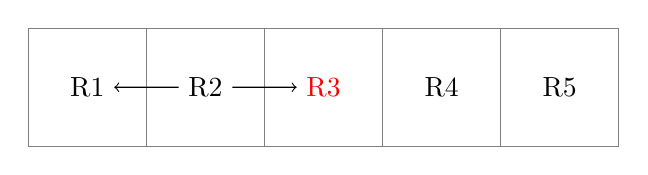
\begin{tikzpicture}[scale = 1.5]
\draw[color = gray] (0,0) grid[xstep = 1cm, ystep = 1cm] (5,1);
\node (R1) at (.5, .5) {R1};
\node (R2) at (1.5,.5) {R2};
\node (R3) [color =  red]  at (2.5,.5) {R3};
\node (R4) at (3.5,.5) {R4};
\node (R5) at (4.5,.5) {R5};
\draw [->] (R2) -- (R1);
\draw [->] (R2) -- (R3);
\end{tikzpicture}
\\
\vspace{1cm}
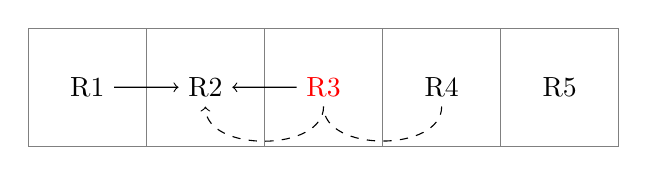
\begin{tikzpicture}[scale = 1.5]
\draw[color = gray] (0,0) grid[xstep = 1cm, ystep = 1cm] (5,1);
\node (R1) at (.5, .5) {R1};
\node (R2) at (1.5,.5) {R2};
\node (R3) [color =  red]  at (2.5,.5) {R3};
\node (R4) at (3.5,.5) {R4};
\node (R5) at (4.5,.5) {R5};
\draw [->] (R1) -- (R2);
\draw [->] (R3) -- (R2);
\draw [->, dashed] (R4) to[out= 270,in=270] (R3) to[out=270,in=270] (R2);
\end{tikzpicture}
\end{figure}

Similarly, the third-order neighbors are: 
\begin{equation*}
\mW^3 = \begin{pmatrix}
      0 & 2 & 0 & 1 & 0 \\
      2 & 0 & 3 & 0 & 1 \\
      0 & 3 & 0 & 3 & 0 \\
      1 & 0 & 3 & 0 & 2 \\
      0 & 1 & 0 & 2 & 1
      \end{pmatrix}
\end{equation*}

Could you explain the elements of this matrix?

%============================================
\section{Examples of Weight Matrices in R}
%============================================

Creating spatial weight matrices manually is a tedious and error-prone process, especially for large datasets. Fortunately, modern statistical software provides robust tools to simplify this task. To start, we typically need a \textbf{shapefile}, a widely used format for storing geographical information.

The shapefile format is a digital vector storage format that supports geometric data types such as points, lines, and polygons, along with associated attributes. It enables diverse representations of geographic data by combining shapes with their corresponding attribute data. A complete shapefile consists of three mandatory files with the following extensions:
\begin{itemize}
  \item \texttt{.shp}: The shape file containing the feature geometry.
  \item \texttt{.shx}: The shape index file, which facilitates fast positional indexing of the feature geometry.
  \item \texttt{.dbf}: The attribute file, formatted in \texttt{dBase} IV format, storing columnar attributes for each shape.
\end{itemize}

These three components must be present for a shapefile to be functional. The \texttt{.shp} file stores the actual geometric data, while the \texttt{.shx} and \texttt{.dbf} files provide supporting information to enable efficient access and attribute storage.

In this example, we demonstrate how to create spatial weight matrices using \proglang{R}. Specifically, we focus on a map of the communes in the Metropolitan Region of Chile. To begin, we load the shapefile into \proglang{R} using the \pkg{sf} package \citep{pabesmasf}, which is designed for handling spatial data.

\begin{knitrout}
\definecolor{shadecolor}{rgb}{0.969, 0.969, 0.969}\color{fgcolor}\begin{kframe}
\begin{alltt}
\hlcom{#Load package sf}
\hlkwd{library}\hldef{(}\hlsng{"sf"}\hldef{)}
\end{alltt}
\end{kframe}
\end{knitrout}

If the shapefile \texttt{mr\_chile.shp} is located in the working directory, we can load it using the \texttt{read\_sf} function:
\begin{knitrout}
\definecolor{shadecolor}{rgb}{0.969, 0.969, 0.969}\color{fgcolor}\begin{kframe}
\begin{alltt}
\hlcom{# Read shape file}
\hldef{mr} \hlkwb{<-} \hlkwd{read_sf}\hldef{(}\hlsng{"mr_chile.shp"}\hldef{)}
\hlkwd{class}\hldef{(mr)}
\end{alltt}
\begin{verbatim}
## [1] "sf"         "tbl_df"     "tbl"        "data.frame"
\end{verbatim}
\end{kframe}
\end{knitrout}

The \code{read\_sf} function reads data from the shapefile into an object of class ``\code{sf}''. The \code{names} function provides the name of the variables in the \texttt{.dbf} file associated with the shape file. 
\begin{knitrout}
\definecolor{shadecolor}{rgb}{0.969, 0.969, 0.969}\color{fgcolor}\begin{kframe}
\begin{alltt}
\hlcom{# Names of the variables in .dbf}
\hlkwd{names}\hldef{(mr)}
\end{alltt}
\begin{verbatim}
##  [1] "ID"         "NAME"       "NAME2"      "URB_POP"    "RUR_POP"   
##  [6] "MALE_POP"   "TOT_POP"    "FEM_POP"    "N_PARKS"    "N_PLAZA"   
## [11] "CONS_HOUSE" "M2_CONS_HA" "GREEN_AREA" "AREA"       "POVERTY"   
## [16] "PER_CONTR_" "PER_HON_SA" "PER_PLANT_" "NURSES"     "DOCTORS"   
## [21] "CONSULT_RU" "CONSULT_UR" "POSTAS"     "ESTAB_MUN_" "PSU_MUN_PR"
## [26] "PSU_PART_P" "PSU_SUB_PR" "STUDENT_SU" "STUDENT_PA" "STUDENT_MU"
## [31] "geometry"
\end{verbatim}
\end{kframe}
\end{knitrout}

Now, let's visualize the shapefile using the \code{plot} function:
\begin{knitrout}
\definecolor{shadecolor}{rgb}{0.969, 0.969, 0.969}\color{fgcolor}\begin{kframe}
\begin{alltt}
\hlcom{# Plot shapefile}
\hlkwd{plot}\hldef{(}\hlkwd{st_geometry}\hldef{(mr),} \hlkwc{main} \hldef{=} \hlsng{"Metropolitan Region-Chile"}\hldef{,} \hlkwc{axes} \hldef{=} \hlnum{TRUE}\hldef{)}
\end{alltt}
\end{kframe}
\end{knitrout}

The metropolitan region with its 52 communes is shown in Figure \ref{fig:plot_mr}.

\begin{figure}[h]
  \caption{Plotting a Map in R}
    \label{fig:plot_mr}
\begin{knitrout}
\definecolor{shadecolor}{rgb}{0.969, 0.969, 0.969}\color{fgcolor}

{\centering \includegraphics[width=9cm,height=9cm]{figure/plot_mr-1} 

}


\end{knitrout}
\end{figure}

%===============================================
\subsection{Creating Contiguity Neighbors}\label{sec:computing-W-in-R}
%===============================================

To construct spatial weight matrices, the \pkg{spdep} package \citep{bivand2013computing} provides an extensive suite of tools. After installation, the package can be loaded as follows:

\begin{knitrout}
\definecolor{shadecolor}{rgb}{0.969, 0.969, 0.969}\color{fgcolor}\begin{kframe}
\begin{alltt}
\hlcom{#Load package}
\hlkwd{library}\hldef{(}\hlsng{"spdep"}\hldef{)}
\end{alltt}
\end{kframe}
\end{knitrout}

In \pkg{spdep}, neighbor relationships between $n$ observations are represented by objects of class \texttt{nb}. These objects are lists of length $n$, where each element is an integer vector containing the indices of neighboring regions. If a region has no neighbors, the corresponding element is assigned an integer value of zero.

The \texttt{poly2nb} function constructs neighbor relationships based on \textbf{contiguity}, generating a neighbors list of class \texttt{nb}. This function supports both the Queen and Rook criteria for defining spatial relationships. Refer to \texttt{help(poly2nb)} for detailed documentation.


As explained in previous section, the Queen criterion defines neighbors as regions that share at least one vertex or edge. The following example demonstrates how to construct a neighbor list for the communes in the Metropolitan Region of Chile:\index{Weight matrix!\texttt{poly2nb} function}

\begin{knitrout}
\definecolor{shadecolor}{rgb}{0.969, 0.969, 0.969}\color{fgcolor}\begin{kframe}
\begin{alltt}
\hlcom{# Create queen W}
\hlkwd{sf_use_s2}\hldef{(}\hlnum{FALSE}\hldef{)}
\hldef{queen.w} \hlkwb{<-} \hlkwd{poly2nb}\hldef{(}\hlkwd{as}\hldef{(mr,} \hlsng{"Spatial"}\hldef{),} \hlkwc{queen} \hldef{=}  \hlnum{TRUE}\hldef{,} \hlkwc{row.names} \hldef{= mr}\hlopt{$}\hldef{NAME)}
\end{alltt}
\end{kframe}
\end{knitrout}

Once the \texttt{nb} object is created, it can be explored using standard methods such as \texttt{print}, \texttt{summary}, and \texttt{plot}. For example, the summary of the Queen-based neighbors list provides information about the spatial relationships:
\begin{knitrout}
\definecolor{shadecolor}{rgb}{0.969, 0.969, 0.969}\color{fgcolor}\begin{kframe}
\begin{alltt}
\hlcom{# Summary of W}
\hlkwd{summary}\hldef{(queen.w)}
\end{alltt}
\begin{verbatim}
## Neighbour list object:
## Number of regions: 52 
## Number of nonzero links: 292 
## Percentage nonzero weights: 10.79882 
## Average number of links: 5.615385 
## Link number distribution:
## 
##  2  3  4  5  6  7  8  9 10 12 
##  3  2  7 15 10 10  2  1  1  1 
## 3 least connected regions:
## Tiltil San Pedro Maria Pinto with 2 links
## 1 most connected region:
## San Bernardo with 12 links
\end{verbatim}
\end{kframe}
\end{knitrout}

The output provides crucial information about the neighbors, including the number of regions (52 communes in this example), the number of nonzero links, the percentage of nonzero weights, the average number of links, and more.

For instance, the commune of San Bernardo stands out as the most connected region with 12 neighbors under the queen scheme. Conversely, the least connected regions are Tiltil, San Pedro, and Maria Pinto, each with only 2 neighbors. The output also shows the distribution of neighbors, revealing that 7 out of 52 regions have 4 neighbors, and only 2 communes have 8 neighbors.

To visualize the region with the largest number of neighbors (San Bernardo) and its immediate neighbors, use the following code:
\begin{knitrout}
\definecolor{shadecolor}{rgb}{0.969, 0.969, 0.969}\color{fgcolor}\begin{kframe}
\begin{alltt}
\hlcom{# Plot communes with largest number of contiguities}
\hldef{cards} \hlkwb{<-} \hlkwd{card}\hldef{(queen.w)}
\hldef{maxconts} \hlkwb{<-} \hlkwd{which}\hldef{(cards} \hlopt{==} \hlkwd{max}\hldef{(cards))}
\hldef{fg} \hlkwb{<-} \hlkwd{rep}\hldef{(}\hlsng{"grey"}\hldef{,} \hlkwd{length}\hldef{(cards))}
\hldef{fg[maxconts]} \hlkwb{<-} \hlsng{"red"}
\hldef{fg[queen.w[[maxconts]]]} \hlkwb{<-} \hlsng{"blue"}
\hlkwd{plot}\hldef{(}\hlkwd{st_geometry}\hldef{(mr),} \hlkwc{col} \hldef{= fg)}
\end{alltt}
\end{kframe}
\end{knitrout}

\begin{figure}[ht]
  \caption{Commune with largest number of contiguities}
    \label{fig:plot_nn}
    \centering
        	\begin{minipage}{1\linewidth}
\begin{knitrout}
\definecolor{shadecolor}{rgb}{0.969, 0.969, 0.969}\color{fgcolor}

{\centering \includegraphics[width=10cm,height=10cm]{figure/neight-1} 

}


\end{knitrout}
\footnotesize
		\emph{Notes:} The commune in red is the spatial unit (San Bernardo) with the largest number of neighbors based on the queen criteria, whereas the communes in blue are its neighbors. 
	\end{minipage}	
\end{figure}

Figure \ref{fig:plot_nn} provides a visual representation where the red-colored commune, San Bernardo, stands out as the spatial unit with the largest number of neighbors according to the queen criteria. Meanwhile, the communes in blue represent its neighboring units.

To transform the \code{list} into an actual matrix $\mW$, we can use the \code{nb2listw} function\index{Weight matrix!\texttt{nb2listw} function}:

\begin{knitrout}
\definecolor{shadecolor}{rgb}{0.969, 0.969, 0.969}\color{fgcolor}\begin{kframe}
\begin{alltt}
\hlcom{# From list to matrix}
\hldef{queen.wl} \hlkwb{<-} \hlkwd{nb2listw}\hldef{(queen.w,} \hlkwc{style} \hldef{=} \hlsng{"W"}\hldef{)}
\hlkwd{summary}\hldef{(queen.wl)}
\end{alltt}
\begin{verbatim}
## Characteristics of weights list object:
## Neighbour list object:
## Number of regions: 52 
## Number of nonzero links: 292 
## Percentage nonzero weights: 10.79882 
## Average number of links: 5.615385 
## Link number distribution:
## 
##  2  3  4  5  6  7  8  9 10 12 
##  3  2  7 15 10 10  2  1  1  1 
## 3 least connected regions:
## Tiltil San Pedro Maria Pinto with 2 links
## 1 most connected region:
## San Bernardo with 12 links
## 
## Weights style: W 
## Weights constants summary:
##    n   nn S0       S1      S2
## W 52 2704 52 19.76751 216.466
\end{verbatim}
\end{kframe}
\end{knitrout}

An important argument for \code{nb2listw} is \code{style}. This argument indicates what type of matrix to create. For example, \code{style = "W"} creates a row-standardize matrix so that $w^s_{ij} = w_{ij}/ \sum_j w_{ij}$. After normalization, each row of $\mW^s$ sums to 1. Other options include \code{"B"} for basic binary coding; \code{"C"} for global standarization, that is, $w^s_{ij} = w_{ij} \cdot (n/ \sum_{i}\sum_j w_{ij})$. If \code{style = "U"}, then $w^s_{ij} = w_{ij}/ \sum_i\sum_j w_{ij}$. In a \code{minmax} matrix, the $(i,j)$th element of $\mW^s$  becomes $w^s_{ij} = w_{ij} / \min\left\lbrace \max_i(\tau_i), \max_i(c_i)\right\rbrace$, with $\max_i(\tau_i)$ being the largest row sum of $\mW$ and $\max_i(c_i)$ being the largest column sum of $\mW$ \citep{kelejian2010specification}. Finally, \code{"S"} is the variance-stabilizing coding scheme where $w^s_{ij} = w_{ij}/ \sqrt{\sum_j w_{ij} ^2}$ \citep{tiefelsdorf1999variance}. 

Additionally, the \code{summary} function provides several constants essential for global spatial autocorrelation statistics, which we will discuss later. 

We can also inspect the attributes of the object using the function \code{attributes}:

\begin{knitrout}
\definecolor{shadecolor}{rgb}{0.969, 0.969, 0.969}\color{fgcolor}\begin{kframe}
\begin{alltt}
\hlcom{# Attributes of wlist}
\hlkwd{attributes}\hldef{(queen.w)}
\end{alltt}
\begin{verbatim}
## $class
## [1] "nb"
## 
## $region.id
##  [1] "Santiago"            "Cerillos"            "Cerro Navia"        
##  [4] "Conchali"            "El Bosque"           "Estacion Central"   
##  [7] "La Cisterna"         "La Florida"          "La Granja"          
## [10] "La Pintana"          "La Reina"            "Lo Espejo"          
## [13] "Lo Prado"            "Macul"               "Nunoa"              
## [16] "Pedro Aguirre Cerda" "Penalolen"           "Providencia"        
## [19] "Quinta Normal"       "Recoleta"            "Renca"              
## [22] "San Joaquin"         "San Miguel"          "San Ramon"          
## [25] "Independencia"       "Puente Alto"         "Las Condes"         
## [28] "Vitacura"            "Quilicura"           "Huechuraba"         
## [31] "Maipu"               "Pudahuel"            "San Bernardo"       
## [34] "Tiltil"              "Lampa"               "Colina"             
## [37] "Lo Barnechea"        "Pirque"              "Paine"              
## [40] "Buin"                "Alhue"               "Melipilla"          
## [43] "San Pedro"           "Maria Pinto"         "Curacavi"           
## [46] "Penaflor"            "Calera de Tango"     "Padre Hurtado"      
## [49] "El Monte"            "Talagante"           "Isla de Maipo"      
## [52] "San Jose de Maipo"  
## 
## $call
## poly2nb(pl = as(mr, "Spatial"), row.names = mr$NAME, queen = TRUE)
## 
## $type
## [1] "queen"
## 
## $snap
## [1] 1.490116e-08
## 
## $sym
## [1] TRUE
## 
## $ncomp
## $ncomp$nc
## [1] 1
## 
## $ncomp$comp.id
##  [1] 1 1 1 1 1 1 1 1 1 1 1 1 1 1 1 1 1 1 1 1 1 1 1 1 1 1 1 1 1 1 1 1 1 1 1 1 1 1
## [39] 1 1 1 1 1 1 1 1 1 1 1 1 1 1
\end{verbatim}
\end{kframe}
\end{knitrout}

Weight matrices based on contiguity are generally symmetric. Use the following command to verify:
\begin{knitrout}
\definecolor{shadecolor}{rgb}{0.969, 0.969, 0.969}\color{fgcolor}\begin{kframe}
\begin{alltt}
\hlcom{# Symmetric W}
\hlkwd{is.symmetric.nb}\hldef{(queen.w)}
\end{alltt}
\begin{verbatim}
## [1] TRUE
\end{verbatim}
\end{kframe}
\end{knitrout}

The Rook criterion considers neighbors that share a common edge. Here's how to construct a Rook-based neighbors list:
\begin{knitrout}
\definecolor{shadecolor}{rgb}{0.969, 0.969, 0.969}\color{fgcolor}\begin{kframe}
\begin{alltt}
\hlcom{# Rook W}
\hldef{rook.w} \hlkwb{<-} \hlkwd{poly2nb}\hldef{(}\hlkwd{as}\hldef{(mr,} \hlsng{"Spatial"}\hldef{),} \hlkwc{row.names} \hldef{= mr}\hlopt{$}\hldef{NAME,} \hlkwc{queen} \hldef{=}  \hlnum{FALSE}\hldef{)}
\hlkwd{summary}\hldef{(rook.w)}
\end{alltt}
\begin{verbatim}
## Neighbour list object:
## Number of regions: 52 
## Number of nonzero links: 272 
## Percentage nonzero weights: 10.05917 
## Average number of links: 5.230769 
## Link number distribution:
## 
##  2  3  4  5  6  7  8  9 10 
##  3  3 12 16  7  6  2  1  2 
## 3 least connected regions:
## Tiltil San Pedro Maria Pinto with 2 links
## 2 most connected regions:
## Santiago San Bernardo with 10 links
\end{verbatim}
\end{kframe}
\end{knitrout}

Finally, we can visualize the spatial connectivity implied by the Queen and Rook criterion using the following set of commands (see Figure \ref{fig:Queen-Rook}). 

\begin{knitrout}
\definecolor{shadecolor}{rgb}{0.969, 0.969, 0.969}\color{fgcolor}\begin{kframe}
\begin{alltt}
\hlcom{# Plot Queen and Rook W Matrices}
\hlkwd{plot}\hldef{(}\hlkwd{st_geometry}\hldef{(mr),} \hlkwc{border} \hldef{=} \hlsng{"grey"}\hldef{)}
\hldef{coords} \hlkwb{<-} \hlkwd{st_coordinates}\hldef{(}\hlkwd{st_centroid}\hldef{(}\hlkwd{st_geometry}\hldef{(mr)))}
\hlkwd{plot}\hldef{(queen.w, coords,} \hlkwc{add} \hldef{=}  \hlnum{TRUE}\hldef{,} \hlkwc{col} \hldef{=} \hlsng{"red"}\hldef{)}
\hlkwd{plot}\hldef{(rook.w, coords,} \hlkwc{add} \hldef{=}  \hlnum{TRUE}\hldef{,} \hlkwc{col} \hldef{=} \hlsng{"yellow"}\hldef{)}
\end{alltt}
\end{kframe}
\end{knitrout}

\begin{figure}[ht]
  \caption{Queen and Rook Criteria for MR}
    \label{fig:Queen-Rook}
\begin{knitrout}
\definecolor{shadecolor}{rgb}{0.969, 0.969, 0.969}\color{fgcolor}

{\centering \includegraphics[width=8cm,height=8cm]{figure/plot-queen-rookT-1} 

}


\end{knitrout}
\end{figure}

%==================================================
\subsection{Creating Distance-based Neighbors}
%==================================================

We proceed to build spatial weight matrices using the $k$-nearest neighbors criteria\index{Weight matrix!\texttt{knearneigh} function}. 

\begin{knitrout}
\definecolor{shadecolor}{rgb}{0.969, 0.969, 0.969}\color{fgcolor}\begin{kframe}
\begin{alltt}
\hlcom{# K-neighbors}
\hlkwd{head}\hldef{(coords,} \hlnum{5}\hldef{)}                                       \hlcom{# show coordinates}
\end{alltt}
\begin{verbatim}
##              X         Y
## [1,] -70.65599 -33.45406
## [2,] -70.71742 -33.50027
## [3,] -70.74504 -33.42278
## [4,] -70.67735 -33.38372
## [5,] -70.67640 -33.56294
\end{verbatim}
\begin{alltt}
\hldef{k1neigh} \hlkwb{<-} \hlkwd{knearneigh}\hldef{(coords,} \hlkwc{k} \hldef{=} \hlnum{1}\hldef{,} \hlkwc{longlat} \hldef{=} \hlnum{TRUE}\hldef{)}  \hlcom{# 1-nearest neighbor}
\hldef{k2neigh} \hlkwb{<-} \hlkwd{knearneigh}\hldef{(coords,} \hlkwc{k} \hldef{=} \hlnum{2}\hldef{,} \hlkwc{longlat} \hldef{=} \hlnum{TRUE}\hldef{)}  \hlcom{# 2-nearest neighbor}
\end{alltt}
\end{kframe}
\end{knitrout}

Here, the \code{coords}\index{Weight matrix!\texttt{coords} function} function extracts spatial coordinates from the shapefile, while \code{knearneigh} returns a matrix containing indices of points belonging to the set of $k$-nearest neighbors for each observation. The \code{k} argument specifies the number of nearest neighbors to return. If the point coordinates are given in longitude-latitude decimal degrees, distances are measured in kilometers when \code{longlat = TRUE}. For \code{longlat = FALSE}, great-circle distances are computed. The resulting objects \code{k1neigh} and \code{k2neigh} are of class \code{knn}.

Inverse distance weight matrices can be computed as follows (see Section \ref{sec:inverse_distance}):

\begin{knitrout}
\definecolor{shadecolor}{rgb}{0.969, 0.969, 0.969}\color{fgcolor}\begin{kframe}
\begin{alltt}
\hlcom{# Inverse weight matrix}
\hldef{dist.mat} \hlkwb{<-} \hlkwd{as.matrix}\hldef{(}\hlkwd{dist}\hldef{(coords,} \hlkwc{method} \hldef{=} \hlsng{"euclidean"}\hldef{))}
\hldef{dist.mat[}\hlnum{1}\hlopt{:}\hlnum{5}\hldef{,} \hlnum{1}\hlopt{:}\hlnum{5}\hldef{]}
\end{alltt}
\begin{verbatim}
##            1          2          3          4          5
## 1 0.00000000 0.07687010 0.09438408 0.07350782 0.11078109
## 2 0.07687010 0.00000000 0.08226867 0.12324109 0.07489489
## 3 0.09438408 0.08226867 0.00000000 0.07814455 0.15606360
## 4 0.07350782 0.12324109 0.07814455 0.00000000 0.17922003
## 5 0.11078109 0.07489489 0.15606360 0.17922003 0.00000000
\end{verbatim}
\begin{alltt}
\hldef{dist.mat.inv} \hlkwb{<-} \hlnum{1} \hlopt{/} \hldef{dist.mat} \hlcom{# 1 / d_\{ij\}}
\hlkwd{diag}\hldef{(dist.mat.inv)} \hlkwb{<-} \hlnum{0}      \hlcom{# 0 in the diagonal}
\hldef{dist.mat.inv[}\hlnum{1}\hlopt{:}\hlnum{5}\hldef{,} \hlnum{1}\hlopt{:}\hlnum{5}\hldef{]}
\end{alltt}
\begin{verbatim}
##           1         2         3         4         5
## 1  0.000000 13.008960 10.595007 13.603994  9.026811
## 2 13.008960  0.000000 12.155295  8.114177 13.352046
## 3 10.595007 12.155295  0.000000 12.796797  6.407644
## 4 13.603994  8.114177 12.796797  0.000000  5.579733
## 5  9.026811 13.352046  6.407644  5.579733  0.000000
\end{verbatim}
\begin{alltt}
\hlcom{# Standardized inverse weight matrix}
\hldef{dist.mat.inve} \hlkwb{<-} \hlkwd{mat2listw}\hldef{(dist.mat.inv,} \hlkwc{style} \hldef{=} \hlsng{"W"}\hldef{,} \hlkwc{row.names} \hldef{= mr}\hlopt{$}\hldef{NAME)}
\hlkwd{summary}\hldef{(dist.mat.inve)}
\end{alltt}
\begin{verbatim}
## Characteristics of weights list object:
## Neighbour list object:
## Number of regions: 52 
## Number of nonzero links: 2652 
## Percentage nonzero weights: 98.07692 
## Average number of links: 51 
## Link number distribution:
## 
## 51 
## 52 
## 52 least connected regions:
## Santiago Cerillos Cerro Navia Conchali El Bosque Estacion Central La Cisterna La Florida La Granja La Pintana La Reina Lo Espejo Lo Prado Macul Nunoa Pedro Aguirre Cerda Penalolen Providencia Quinta Normal Recoleta Renca San Joaquin San Miguel San Ramon Independencia Puente Alto Las Condes Vitacura Quilicura Huechuraba Maipu Pudahuel San Bernardo Tiltil Lampa Colina Lo Barnechea Pirque Paine Buin Alhue Melipilla San Pedro Maria Pinto Curacavi Penaflor Calera de Tango Padre Hurtado El Monte Talagante Isla de Maipo San Jose de Maipo with 51 links
## 52 most connected regions:
## Santiago Cerillos Cerro Navia Conchali El Bosque Estacion Central La Cisterna La Florida La Granja La Pintana La Reina Lo Espejo Lo Prado Macul Nunoa Pedro Aguirre Cerda Penalolen Providencia Quinta Normal Recoleta Renca San Joaquin San Miguel San Ramon Independencia Puente Alto Las Condes Vitacura Quilicura Huechuraba Maipu Pudahuel San Bernardo Tiltil Lampa Colina Lo Barnechea Pirque Paine Buin Alhue Melipilla San Pedro Maria Pinto Curacavi Penaflor Calera de Tango Padre Hurtado El Monte Talagante Isla de Maipo San Jose de Maipo with 51 links
## 
## Weights style: W 
## Weights constants summary:
##    n   nn S0       S1       S2
## W 52 2704 52 2.902384 214.3332
\end{verbatim}
\end{kframe}
\end{knitrout}

The \code{dist} function from the \pkg{stats} package computes the distance matrix using the specified metric---Euclidean distance in this example. Other available methods include \code{maximum}, \code{manhattan}, \code{canberra}, \code{binary}, and \code{minkowski}. The \code{mat2listw} function converts a square spatial weight matrix into a list format suitable for spatial analysis. For additional details on spatial weight matrices, see \cite{stewart2010choosing}.

The following code demonstrates how to plot different weight matrices:

\begin{knitrout}
\definecolor{shadecolor}{rgb}{0.969, 0.969, 0.969}\color{fgcolor}\begin{kframe}
\begin{alltt}
\hlcom{# Plot Weights}
\hlkwd{par}\hldef{(}\hlkwc{mfrow} \hldef{=} \hlkwd{c}\hldef{(}\hlnum{2}\hldef{,} \hlnum{2}\hldef{))}
\hlkwd{plot}\hldef{(}\hlkwd{st_geometry}\hldef{(mr),} \hlkwc{border} \hldef{=} \hlsng{"grey"}\hldef{,} \hlkwc{main} \hldef{=} \hlsng{"Queen"}\hldef{)}
\hlkwd{plot}\hldef{(queen.w, coords,} \hlkwc{add} \hldef{=}  \hlnum{TRUE}\hldef{,} \hlkwc{col} \hldef{=} \hlsng{"red"}\hldef{)}
\hlkwd{plot}\hldef{(}\hlkwd{st_geometry}\hldef{(mr),} \hlkwc{border} \hldef{=} \hlsng{"grey"}\hldef{,} \hlkwc{main} \hldef{=} \hlsng{"1-Neigh"}\hldef{)}
\hlkwd{plot}\hldef{(}\hlkwd{knn2nb}\hldef{(k1neigh), coords,} \hlkwc{add} \hldef{=} \hlnum{TRUE}\hldef{,} \hlkwc{col} \hldef{=} \hlsng{"red"}\hldef{)}
\hlkwd{plot}\hldef{(}\hlkwd{st_geometry}\hldef{(mr),} \hlkwc{border} \hldef{=} \hlsng{"grey"}\hldef{,} \hlkwc{main} \hldef{=} \hlsng{"2-Neigh"}\hldef{)}
\hlkwd{plot}\hldef{(}\hlkwd{knn2nb}\hldef{(k2neigh), coords,} \hlkwc{add} \hldef{=} \hlnum{TRUE}\hldef{,} \hlkwc{col} \hldef{=} \hlsng{"red"}\hldef{)}
\hlkwd{plot}\hldef{(}\hlkwd{st_geometry}\hldef{(mr),} \hlkwc{border} \hldef{=} \hlsng{"grey"}\hldef{,} \hlkwc{main} \hldef{=} \hlsng{"Inverse Distance"}\hldef{)}
\hlkwd{plot}\hldef{(dist.mat.inve, coords,} \hlkwc{add} \hldef{=}  \hlnum{TRUE}\hldef{,} \hlkwc{col} \hldef{=} \hlsng{"red"}\hldef{)}
\end{alltt}
\end{kframe}
\end{knitrout}


\begin{figure}[h!]
  \caption{Different Spatial Weight Schemes for MR}
    \label{fig:more_ws}
\begin{knitrout}
\definecolor{shadecolor}{rgb}{0.969, 0.969, 0.969}\color{fgcolor}

{\centering \includegraphics[width=\maxwidth]{figure/plot-all-wsT-1} 

}


\end{knitrout}
\end{figure}

\subsection{Constructing a Spatially Lagged Variable}

Spatially lagged variables play a crucial role in various spatial tests and regression specifications. In the \pkg{spdep} package, these variables are crEATED using the  \code{lag.listw} function.

Let's begin by combining the variables  \code{POVERTY} and \code{URB\_POP} into a matrix and check the contents with \code{head}:
\begin{knitrout}
\definecolor{shadecolor}{rgb}{0.969, 0.969, 0.969}\color{fgcolor}\begin{kframe}
\begin{alltt}
\hlcom{# X matrix}
\hldef{X} \hlkwb{<-} \hlkwd{cbind}\hldef{(mr}\hlopt{$}\hldef{POVERTY, mr}\hlopt{$}\hldef{URB_POP)}
\hlkwd{head}\hldef{(X,} \hlnum{5}\hldef{)}
\end{alltt}
\begin{verbatim}
##      [,1]   [,2]
## [1,]    8 159919
## [2,]    9  65262
## [3,]   18 131850
## [4,]   12 104634
## [5,]   14 166514
\end{verbatim}
\end{kframe}
\end{knitrout}

Now, we can generate a spatially lagged version of this matrix, using the \code{queen.w} weights\index{Weight matrix!\texttt{lag.listw} function}:

\begin{knitrout}
\definecolor{shadecolor}{rgb}{0.969, 0.969, 0.969}\color{fgcolor}\begin{kframe}
\begin{alltt}
\hlcom{# Create WX}
\hldef{WX} \hlkwb{<-} \hlkwd{lag.listw}\hldef{(}\hlkwd{nb2listw}\hldef{(queen.w), X)}
\hlkwd{head}\hldef{(WX)}
\end{alltt}
\begin{verbatim}
##          [,1]     [,2]
## [1,]  9.10000 100138.9
## [2,] 12.40000 299498.4
## [3,] 14.00000 144756.5
## [4,] 14.60000 121974.2
## [5,] 18.25000 170266.5
## [6,] 10.42857 236231.1
\end{verbatim}
\end{kframe}
\end{knitrout}


%****************************************************
\section{Testing for Spatial Autocorrelation}
%*****************************************************

As introduced in Section \ref{sec:Spatial_autocorrelation}, spatial autocorrelation refers to the relationship between the values of a variable across space. Positive spatial autocorrelation arises when similar values cluster together—high values near high values or low values near low values. In contrast, negative spatial autocorrelation reflects spatial dispersion, where high values are surrounded by low values, or vice versa.

A central empirical question is whether the observed spatial pattern reflects a true spatial process or is simply the result of random chance. Formal hypothesis tests are therefore necessary to evaluate whether the value of a variable at one location is statistically dependent on the values observed at neighboring locations.


%=============================================================
\subsection{Global Spatial Autocorrelation: Moran's I}\label{sec:moransI}
%============================================================

Global spatial autocorrelation measures the overall degree of spatial clustering or dispersion in a dataset. These indices evaluate the similarity between values at different locations $i$ and $j$, weighted by a spatial proximity matrix. High similarity in close proximity suggests clustering, while dissimilar values nearby imply spatial dispersion.

The most widely used measure of global spatial autocorrelation is \textbf{Moran's I}.\footnote{Other measures, such as Geary's $C$, are also available, but this section focuses on Moran's I due to its popularity and interpretability.} Moran's I tests the null hypothesis of spatial randomness and quantifies the extent of global spatial association.

Moran's I is given by\index{Moran's I test}:
\begin{equation}\label{eq:I-moran}
I = \frac{\sum_{i = 1}^n\sum_{j=1, j\neq i}^n w_{ij}\left(x_i - \bar{x}\right)\left(x_j - \bar{x}\right)}{S_0 \sum_{i = 1}^n\left(x_i - \bar{x}\right)^2/n} = \frac{n\sum_{i = 1}^n\sum_{j=1}^n w_{ij}\left(x_i - \bar{x}\right)\left(x_j - \bar{x}\right)}{S_0 \sum_{i = 1}^n\left(x_i - \bar{x}\right)^2},
\end{equation}
%
where $w_{ij}$ denotes the spatial weight between regions $i$ and $j$, and $S_0 = \sum_{i=1}^n\sum_{j=1}^n w_{ij}$ is the sum of all spatial weights.

In matrix notation, this can be expressed as:
\begin{equation*}
	I = \frac{n}{S_0} \frac{\vz^\top\mW\vz}{\vz^\top\vz},
\end{equation*}
%
where: 
\begin{equation*}
\vz = \begin{pmatrix}
          x_1 - \bar{x}\\
          x_2 - \bar{x} \\
          \vdots\\
          x_n - \bar{x}
      \end{pmatrix}.
\end{equation*}

If $\mW$ is row-standardized, then $S_0 = n$, and the expression simplifies to:
\begin{equation*}
I = \frac{\vz^\top \mW^s \vz}{\vz^\top \vz}.
\end{equation*}

Moran’s I ranges from $-1$ (perfect dispersion) to $+1$ (perfect clustering). A value close to zero suggests spatial randomness.


A helpful graphical tool for interpreting Moran’s I is the \textbf{Moran Scatterplot}. It plots the standardized values of a variable (horizontal axis) against the standardized spatial lag (vertical axis), i.e., the average value of neighboring units (see Figure \ref{fig:moran_scatterplot}). As noted by \citet{anselin1996chapter}, standardizing both axes (mean zero, variance one) allows visualization of both global and local spatial autocorrelation. The slope of the best-fit line corresponds to Moran’s I, while each quadrant reveals different types of local spatial association.

The quadrants of the Moran Scatterplot indicate:

\begin{itemize}
  \item \textbf{Quadrant I (High-High)}: Regions with above-average values surrounded by neighbors also above average.
  \item \textbf{Quadrant II (Low-High)}: Regions with below-average values surrounded by neighbors with above-average values.
  \item \textbf{Quadrant III (Low-Low)}: Regions with below-average values surrounded by similarly low neighbors.
  \item \textbf{Quadrant IV (High-Low)}: Regions with above-average values surrounded by below-average neighbors.
\end{itemize}

Quadrants I and III reflect \textbf{positive spatial autocorrelation} (clustering of similar values), while Quadrants II and IV reflect \textbf{negative spatial autocorrelation} (clustering of dissimilar values).

\begin{figure}[ht]
  \caption{Moran Scatterplot}\label{fig:moran_scatterplot}
\begin{knitrout}
\definecolor{shadecolor}{rgb}{0.969, 0.969, 0.969}\color{fgcolor}

{\centering \includegraphics[width=\maxwidth]{figure/moran-1} 

}


\end{knitrout}
\end{figure}


To grasp the essence of Moran's I, it is essential to draw parallels with the Ordinary Least Squares (OLS) coefficient. Recall the OLS coefficient formula:
\begin{equation*}
  \widehat{\beta}= \frac{\sum_{i = 1}^n\left(x_i - \bar{x}\right)(y_i - \bar{y})}{\sum_{i = 1}^n \left(x_i - \bar{x}\right)^2}
\end{equation*}

Now, examining Equation \eqref{eq:I-moran}, Moran's I equates to the slope coefficient of a linear regression, where the spatial lag $\mW\vx$ is regressed on the observation vector $\vx$, both measured in deviation from their means. It's worth noting that Moran's I is not equivalent to the slope of $\vx$ on $\mW\vx$, which might seem more intuitive.

The hypothesis tested by the Moran's $I$ is the following:
\begin{itemize}
  \item $H_0$: $\vx$ is spatially independent; the observed $\vx$ is assigned at random among locations. In this case, $I$ is close to zero.
  \item $H_1$: $\vx$ is not spatially independent. In this case $I$ is statistically different from zero. 
\end{itemize}

Now, considering the distribution of Moran's I, our interest lies in the distribution of:
\begin{equation*}
  \frac{I - \E\left[I\right]}{\sqrt{\var(I)}}.
\end{equation*}

There are two methods to compute the mean and variance of Moran's I. The first assumes a normal distribution for $x_i$, while the second involves randomization of $x_i$. Under the normal assumption, it is assumed that the random variable $x_i$ results from $n$ independent draws from a normal population. Conversely, under the randomization assumption, irrespective of the underlying distribution of populations, observed values of $x_i$ are repeatedly and randomly permuted.

\subsubsection{Moments Under Normality Assumption}

Theorem \ref{teo:Moran_normal} gives the moments of Moran's I under normality. 

%%%%%%%%%%%%%%%%%%%%%%%%%%%%%%%%%%%%%%%
\begin{theorem}[Moran's $I$ Under Normality]\label{teo:Moran_normal}\index{Moran's I test!Normality}
Assume that $\left\lbrace \vx_i\right\rbrace = \left\lbrace x_1, x_2,\ldots, x_n\right\rbrace$ are independent and distributed as $\rN(\mu, \sigma^2)$, but $\mu$ and $\sigma^2$ are unknown. Then:
\begin{equation*}
\E\left(I\right) = - \frac{1}{n - 1}, 
\end{equation*}
%
and
\begin{equation*}
\E\left(I^2\right) = \frac{n^2S_1 - nS_2 + 3S_0^2}{S_0^2(n^2 - 1)},
\end{equation*}
%
where $S_0=\sum_{i = 1}^n\sum_{j=1}^nw_{ij}$, $S_1= \sum_{i = 1}^n\sum_{j = 1}^n(w_{ij} + w_{ji})^2/2$, $S_2 = \sum_{i = 1}^n(w_{i.} + w_{.i})^2$, where $w_{i.}= \sum_{j = 1}^nw_{ij}$ and $w_{i.}=\sum_{j = 1}^nw_{ji}$
Then:
\begin{equation*}
\var\left(I\right)=\E\left(I^2\right) - \E\left(I\right)^2.
\end{equation*}
\end{theorem}
%%%%%%%%%%%%%%%%%%%%%%%%%%%%%%%%%%%%%%%%

% %----------------------------------------
% \begin{proof}
% Let $z_i=x_i - \bar{x}$. Under normality of $x_i$, the following moments are true for $z_i$:
% \begin{eqnarray*}
% \E\left[z_i\right]   & = & 0, \\
% \E\left[z_i^2\right] & = & \sigma^2 - \frac{\sigma^2}{n}, \\
% \E\left[z_iz_j\right] & = & - \frac{\sigma^2}{n} \\
% \E\left[z_i^2 z_j^2\right] & = & \frac{(n^2 - 2n + 3)\sigma^2}{m^2}, \\
% \E\left[z_i^2 z_jz_k\right] & = & - \frac{(n -3)\sigma^4}{n}, \\
% \E\left[z_iz_jz_kz_l\right] & = & \frac{3 \sigma^4}{n^2}.
% \end{eqnarray*}
% 
% Then:
% \begin{equation}
%   \begin{aligned}
%     \E\left[I\right] & = \frac{n}{S_0}\frac{\E\left[\sum_{i = 1}^n\sum_{j=1}^nw_{ij}z_iz_j\right]}{\E\left[\sum_{i=1}^nz_i^2\right]}
%     & = \frac{n}{S_0}\sum_{i = 1}^n\sum_{j=1}^nw_{ij}\frac{\E\left[z_iz_j\right]}{\sum_{i=1}^n\E\left[z_i^2\right]} \\
%     & = \frac{-nS_0\frac{\sigma^2}{n}}{S_0 n (1 - 1/n)\sigma^2 } \\
%     & = -\frac{\frac{\sigma^2}{n}}{(1 - 1/n)\sigma^2 } \\
%     & = -\frac{1}{n - 1} 
%   \end{aligned}
% \end{equation}
% %
% and
% \begin{equation}
%   \begin{aligned}
%     \E\left[I^2\right] & = \E\left[\frac{n^2}{S_0^2}\frac{\left[\sum_{i = 1}^n\sum_{j=1}^nw_{ij}z_iz_j\right]^2}{\left[\sum_{i=1}^nz_i^2\right]^2}\right] \\
%     & = \frac{n^2}{S_0^2} \E\left[\frac{1/2\sum_{(2)}(w_{ij} + w_{ji})^2 z_i^2 z_j^2 + \sum_{(3)}(w_{ij} + w_{ji})(w_{ik} + w_{ki})z_i^2z_jz_k + \sum_{(4)} w_{ij}w_{kl}z_iz_jz_kz_l}{s}\right]
%   \end{aligned}
% \end{equation}
% \end{proof}
% %----------------------------------------

\subsubsection{Moran's $I$ under Randomization}

%Recall that when testing a null hypothesis we need a test statistic that will have different values under the null hypothesis and the alternatives. We then need to compute the sampling distribution of the test statistic when the null hypothesis is true. For some test statistics and some null hypotheses this can be done analytically. Then, the $p$-value is the probability that the test statistic would be at least as extreme as we observed, if the null hypothesis is true.

%A permutation test gives a simple way to compute the sampling distribution for any test statistic. 

%To estimate the sampling distribution of the test statistic we need many samples generated under the strong null hypothesis. A permutation test builds sampling distribution by resampling the observed data. Specifically, we can ``shuffle'' or permute the observed data by 


%A randomization test (also called a permutation test) is a type of statistical significance test in which the distribution of the test statistic under the null hypothesis is obtained by calculating all possible values of the test statistics under rearrangements of the labels on the observed points. 

%No matter what the underlying distribution of the population, we consider the observed values of $x_i$ were repeatedly randomly permuted.


%Under randomization 

%The testing method under randomization assumption is called permutation test. 

Theorem \ref{teo:Moran_random} gives the moments of Moran's I under randomization. 

%%%%%%%%%%%%%%%%%%%%%%%%%%%%%%%%
\begin{theorem}[Moran's $I$ Under Randomization]\label{teo:Moran_random}\index{Moran's I test!Randomization}
Under permutation, we have:
\begin{equation*}
\E\left(I\right) = - \frac{1}{n - 1}, 
\end{equation*}
%
and
\begin{equation*}
\E\left(I^2\right) = \frac{n\left[\left(n^2 - 3n + 3\right)S_1 - nS_2 + 3S_0^2\right]-b_2\left[\left(n^2 - n\right)S_1 - 2nS_2 + 6S_0^2\right]}{(n-1)(n-2)(n-3)S_0^2},
\end{equation*}
%
where $S_0=\sum_{i = 1}^n\sum_{j=1}^nw_{ij}$, $S_1= \sum_{i = 1}^n\sum_{j = 1}^n(w_{ij} + w_{ji})^2/2$, $S_2 = \sum_{i = 1}^n(w_{i.} + w_{.i})^2$, where $w_{i.}= \sum_{j = 1}^nw_{ij}$ and $w_{i.}=\sum_{j = 1}^nw_{ji}$.Then:
\begin{equation*}
\var\left(I\right)=\E\left(I^2\right) - \E\left(I\right)^2
\end{equation*}
\end{theorem}
%%%%%%%%%%%%%%%%%%%%%%%%%%%%%%%

It is important to note that the expected value of Moran's $I$ under normality and randomization is the same. 

\subsubsection{Monte Carlo Moran's $I$}

The normality assumption is a very strong assumption. However we can use the Moran’s I test based on Monte Carlo simulation.

The essence of any Monte Carlo test, especially for Moran's I, involves the following steps\index{Moran's I test!Monte carlo}: 

\begin{itemize}
  \item Specify a test statistic $T$ for which large values indicate evidence against the null hypothesis $H_0$ (no spatial autocorrelation).
  \item  Given an observed value $t_{obs}$ of the test statistic, compute the p-value as $\Pr(T\geq t_{obs}|H_0)$. This involves understanding the distribution of $T$ under the assumption of $H_0$.
\end{itemize}

The algorithm for the Moran's I Monte Carlo test is as follows:

%-------------------------------------------------------
\begin{algorithm}[Moran's' I Monte Carlo Test]
The procedure is the following:
\begin{enumerate}
\item Rearrange the spatial data by shuffling their location and compute the Moran's I $S$ times. This will create the distribution under $H_0$. This operationalizes spatial randomness. 
\item Let $I_1^*, I_2^*,\ldots, I_S^*$ be the Moran's I for each time. A consistent Monte Carlo p-value is then:
  \begin{equation*}
    \widehat{p} = \frac{1 + \sum_{s=1}^S 1(I^*_s \geq I_{obs})}{S + 1}
  \end{equation*}
  \item For tests at the $\alpha$ level or at $100(1- \alpha)\%$ confidence intervals, there are reasons for choosing $S$ so that $\alpha(S + 1)$ is an integer. For example, use $S=999$ for confidence intervals and hypothesis tests when $\alpha = 0.05$.
\end{enumerate}
\end{algorithm}
%-------------------------------------------------------

%%=====================================================
%\subsection{Local Indicators of Spatial Association (LISA)}
%=====================================================

%\cite{anselin1995local} suggests that a local indicator of spatial association (LISA) is any statistic that satisfies the following two requirements:

%\begin{enumerate}
%  \item the LISA for each observation gives an indication of the extent of significant spatial clustering of similar values around that observation;
%  \item the sum of LISAs for all observations is proportional to a global indicator of spatial association.
%\end{enumerate}

%=====================================================
\section{Application: Poverty in Santiago, Chile}
%=====================================================

In this section, we conduct an Exploratory Spatial Data Analysis (ESDA) of poverty in the Metropolitan Region of Chile.


%================================
\subsection{Cloropeth Graphs}
%================================

To understand the spatial variation in poverty, a natural starting point is to visualize its geographic distribution. Such visualizations serve multiple purposes. National or aggregate indicators often mask significant disparities across smaller spatial units, such as communes. Poverty mapping allows us to uncover and highlight these localized differences. In addition, maps are powerful tools for communicating complex spatial information in an intuitive and accessible way.

We begin by generating a choropleth map\footnote{The term choropleth originates from the Greek words choros (space) and pleth (value).} using the \verb|plot| function. Specifically, we employ a quantile classification scheme, in which the range of the poverty variable is divided into intervals containing an equal number of spatial units. This facilitates comparisons across areas with varying levels of poverty by grouping them into ranked categories.

\begin{knitrout}
\definecolor{shadecolor}{rgb}{0.969, 0.969, 0.969}\color{fgcolor}\begin{kframe}
\begin{alltt}
\hlcom{# Cloropleth graphs ----}
\hlkwd{library}\hldef{(}\hlsng{"RColorBrewer"}\hldef{)}
\hlkwd{plot}\hldef{(mr[}\hlsng{"POVERTY"}\hldef{],}
       \hlkwc{breaks} \hldef{=} \hlsng{"quantile"}\hldef{,}
       \hlkwc{nbreaks} \hldef{=} \hlnum{5}\hldef{,}
       \hlkwc{pal} \hldef{=} \hlkwd{brewer.pal}\hldef{(}\hlnum{5}\hldef{,} \hlsng{"Blues"}\hldef{),}
       \hlkwc{main} \hldef{=} \hlsng{""}\hldef{,}
       \hlkwc{axes} \hldef{=} \hlnum{TRUE}\hldef{)}
\end{alltt}
\end{kframe}
\end{knitrout}

Figure \ref{fig:cloro-graph} provides valuable insights into the spatial structure of poverty in the Metropolitan Region. First, it reveals that poverty is not uniformly distributed across the territory. Instead, there are marked differences in poverty levels among communes. Second, the map demonstrates the added value of disaggregated spatial indicators. For example, it becomes evident that poverty is more pronounced in central communes, while peripheral areas tend to have lower levels of poverty—an insight that would be obscured in aggregate regional statistics.


\begin{figure}
\caption{Cloropleth map: Poverty in the Metropolitan Region}\label{fig:cloro-graph}
\begin{knitrout}
\definecolor{shadecolor}{rgb}{0.969, 0.969, 0.969}\color{fgcolor}

{\centering \includegraphics[width=\maxwidth]{figure/cloro-graphs-1} 

}


\end{knitrout}
\end{figure}

In a quantile classification, data values are ranked and divided into intervals such that each class contains the same number of observations. This approach is particularly useful for comparing spatial units on a relative scale. Since each color represents an equal share of the data, quantile maps are easy to interpret and visually balanced, though they may sometimes exaggerate differences when the underlying data distribution is skewed.

While the visual inspection of poverty's spatial distribution in Figure~\ref{fig:cloro-graph} offers preliminary insights, it is important to recognize the sensitivity of such graphical analysis to arbitrary decisions---such as the number and boundaries of classification intervals. Therefore, a more formal statistical approach is necessary to evaluate whether the observed spatial pattern is the result of a genuinely spatial process or simply due to random variation.

To this end, we employ Moran's I test to formally assess the presence of spatial autocorrelation in the distribution of poverty.


%================================
\subsection{Moran's I Test}
%================================

We begin by constructing two types of spatial weight matrices—queen and rook contiguity—to evaluate the robustness of the test under alternative neighborhood definitions:

\begin{knitrout}
\definecolor{shadecolor}{rgb}{0.969, 0.969, 0.969}\color{fgcolor}\begin{kframe}
\begin{alltt}
\hlcom{# Generate W matrices}
\hldef{queen.w} \hlkwb{<-} \hlkwd{poly2nb}\hldef{(}\hlkwd{as}\hldef{(mr,} \hlsng{"Spatial"}\hldef{),} \hlkwc{row.names} \hldef{= mr}\hlopt{$}\hldef{NAME,} \hlkwc{queen} \hldef{=}  \hlnum{TRUE}\hldef{)}
\hldef{rook.w}  \hlkwb{<-} \hlkwd{poly2nb}\hldef{(}\hlkwd{as}\hldef{(mr,} \hlsng{"Spatial"}\hldef{),} \hlkwc{row.names} \hldef{= mr}\hlopt{$}\hldef{NAME,} \hlkwc{queen} \hldef{=}  \hlnum{FALSE}\hldef{)}
\end{alltt}
\end{kframe}
\end{knitrout}

Moran’s I test for spatial autocorrelation is implemented in the \pkg{spdep} package \citep{spdep}. There are two main functions for conducting this test:

\begin{itemize}
\item  \code{moran.test}: performs the test under either a normality or randomization assumption;\index{Moran's I test!\texttt{moran.test} function}
\item  \code{moran.mc}: computes a permutation-based test using Monte Carlo simulations.\index{Moran's I test!\texttt{moran.mc} function}
\end{itemize}

The code below performs the test under the normality assumption (i.e., setting \code{randomisation = FALSE}) for both weight matrices:

\begin{knitrout}
\definecolor{shadecolor}{rgb}{0.969, 0.969, 0.969}\color{fgcolor}\begin{kframe}
\begin{alltt}
\hlcom{# Moran's I test}
\hlkwd{moran.test}\hldef{(mr}\hlopt{$}\hldef{POVERTY,} \hlkwc{listw} \hldef{=} \hlkwd{nb2listw}\hldef{(queen.w),} \hlkwc{randomisation} \hldef{=} \hlnum{FALSE}\hldef{,}
           \hlkwc{alternative} \hldef{=} \hlsng{'two.sided'}\hldef{)}
\end{alltt}
\begin{verbatim}
## 
## 	Moran I test under normality
## 
## data:  mr$POVERTY  
## weights: nb2listw(queen.w)    
## 
## Moran I statistic standard deviate = 4.0453, p-value = 5.225e-05
## alternative hypothesis: two.sided
## sample estimates:
## Moran I statistic       Expectation          Variance 
##       0.306497992      -0.019607843       0.006498517
\end{verbatim}
\begin{alltt}
\hlkwd{moran.test}\hldef{(mr}\hlopt{$}\hldef{POVERTY,} \hlkwc{listw} \hldef{=} \hlkwd{nb2listw}\hldef{(rook.w),} \hlkwc{randomisation} \hldef{=} \hlnum{FALSE}\hldef{,}
           \hlkwc{alternative} \hldef{=} \hlsng{'two.sided'}\hldef{)}
\end{alltt}
\begin{verbatim}
## 
## 	Moran I test under normality
## 
## data:  mr$POVERTY  
## weights: nb2listw(rook.w)    
## 
## Moran I statistic standard deviate = 4.3309, p-value = 1.485e-05
## alternative hypothesis: two.sided
## sample estimates:
## Moran I statistic       Expectation          Variance 
##       0.342282943      -0.019607843       0.006982432
\end{verbatim}
\end{kframe}
\end{knitrout}

By default, \code{moran.test} uses a one-sided test and the randomization assumption. To obtain a two-sided test under the normal approximation, we must explicitly set \code{randomisation = FALSE} and \code{alternative = 'two.sided'}. Note also that the option \code{zero.policy = FALSE} implies that spatial units with no neighbors (islands) will yield \code{NA}; setting this option to \code{TRUE} assigns them a spatial lag value of zero.

The test results reveal that Moran’s I is approximately 0.30 (queen) and 0.34 (rook), both highly significant. This provides strong evidence of positive spatial autocorrelation in poverty rates, i.e., communes with similar levels of poverty tend to be located near each other.


\begin{remark}
When applying Moran’s I to different variables using the same spatial weight matrix, the expected value and variance of the test statistic under the normal approximation remain unchanged. Why? Because under normality, the expectation and variance depend only on the spatial structure (i.e., the weights matrix), not the values of the variable.
\end{remark}

We now replicate the test under the randomization assumption, which treats the observed poverty values as a random permutation of fixed values across space:

\begin{knitrout}
\definecolor{shadecolor}{rgb}{0.969, 0.969, 0.969}\color{fgcolor}\begin{kframe}
\begin{alltt}
\hlcom{# Moran test under randomization}
\hlkwd{moran.test}\hldef{(mr}\hlopt{$}\hldef{POVERTY,} \hlkwc{listw} \hldef{=} \hlkwd{nb2listw}\hldef{(queen.w),}
           \hlkwc{alternative} \hldef{=} \hlsng{'two.sided'}\hldef{)}
\end{alltt}
\begin{verbatim}
## 
## 	Moran I test under randomisation
## 
## data:  mr$POVERTY  
## weights: nb2listw(queen.w)    
## 
## Moran I statistic standard deviate = 4.0689, p-value = 4.723e-05
## alternative hypothesis: two.sided
## sample estimates:
## Moran I statistic       Expectation          Variance 
##       0.306497992      -0.019607843       0.006423226
\end{verbatim}
\end{kframe}
\end{knitrout}

Note that the value of the Moran’s I statistic and its expected value remain the same as in the normal case. However, the variance differs, leading to a different test statistic and $p$-value.

To implement a Monte Carlo version of the test, we use \code{moran.mc}, which requires specifying the number of permutations \code{nsim}. Best practices suggest using a number ending in 9 (e.g., 99 or 999), as this leads to pseudo $p$-values that round to familiar significance levels:


\begin{knitrout}
\definecolor{shadecolor}{rgb}{0.969, 0.969, 0.969}\color{fgcolor}\begin{kframe}
\begin{alltt}
\hlcom{# Moran's Test}
\hlkwd{set.seed}\hldef{(}\hlnum{1234}\hldef{)}
\hlkwd{moran.mc}\hldef{(mr}\hlopt{$}\hldef{POVERTY,} \hlkwc{listw} \hldef{=} \hlkwd{nb2listw}\hldef{(queen.w),}
           \hlkwc{nsim} \hldef{=} \hlnum{99}\hldef{)}
\end{alltt}
\begin{verbatim}
## 
## 	Monte-Carlo simulation of Moran I
## 
## data:  mr$POVERTY 
## weights: nb2listw(queen.w)  
## number of simulations + 1: 100 
## 
## statistic = 0.3065, observed rank = 100, p-value = 0.01
## alternative hypothesis: greater
\end{verbatim}
\end{kframe}
\end{knitrout}

The result shows that none of the permuted datasets produced a Moran’s I greater than the observed value of 0.3065, resulting in a pseudo $p$-value of $(0 + 1)/(99 + 1) = 0.01$.

We can also visualize the test using the Moran scatterplot, which plots each unit’s value against its spatial lag:

\begin{knitrout}
\definecolor{shadecolor}{rgb}{0.969, 0.969, 0.969}\color{fgcolor}\begin{kframe}
\begin{alltt}
\hlcom{# Moran's plot}
\hlkwd{moran.plot}\hldef{(mr}\hlopt{$}\hldef{POVERTY,} \hlkwc{listw} \hldef{=} \hlkwd{nb2listw}\hldef{(queen.w))}
\end{alltt}
\end{kframe}
\end{knitrout}

\begin{figure}[ht]
\caption{Moran Plot for Poverty}\label{fig:mp-poverty}
\begin{knitrout}
\definecolor{shadecolor}{rgb}{0.969, 0.969, 0.969}\color{fgcolor}

{\centering \includegraphics[width=\maxwidth]{figure/moran-plotT-1} 

}


\end{knitrout}
\end{figure}

Figure~\ref{fig:mp-poverty} shows that most communes fall in Quadrants I and III, suggesting strong positive spatial autocorrelation: areas with high (low) poverty tend to be near others with high (low) poverty. Exceptions are visible in Quadrants II and IV. For example, San Miguel displays low poverty despite being surrounded by high-poverty neighbors.

A major limitation of Moran’s I is that it only captures global spatial autocorrelation. While it indicates whether spatial clustering exists overall, it does not identify where such clusters or outliers occur. To investigate local patterns of spatial dependence, local indicators of spatial association (LISA) are needed.

%-----------------------
\section{Exercises}
%-------------------

\begin{exercises}
 \exercise Another method used for creating spatial weight matrices in Monte Carlo studies is the ``$k$-ahead and $k$-behind'' criterion in a circular world. (This was introduced by \cite{kelejian1999generalized}). In this approach, each spatial unit is assumed to have $k$ neighbors which are ahead of it in the order of sample, and $k$ units which are behind it. The number $k$ is typically chosen to be small relative to the sample size. Thus, each spatial unit has $2k$ neighbors. Weighting matrices which are built on this framework are typically row normalized, and all of the nonzero elements in the matrix are $1/(2k)$. Suppose $n =10$ and $k =2$. Specify the third row of the $10\times 10$ weighting matrix.\label{exercise:k-ahead}
 \exercise For a general sample size, say $n$, which corresponds to a checkerboard of squares, what is the minimum number of neighbors a unit can have if the weighting matrix is based on a queen pattern?
 \exercise  Let $INC_r$ denote the per capita income in cross-sectional unit $r = 1, \ldots, n$. Consider the following definition for the spatial weight $w_{ij}$:
	\begin{equation*}
	w_{ij}= \alpha\left[1 - \frac{\left|INC_i - INC_j\right|}{INC_i+ INC_j}\right], 
	\end{equation*}
	%
	where $\alpha > 0$ is a fixed positive constant. Show that the constant $\alpha$ cancels out when the weight matrix $\mW = [w_{ij}]$ is row-standardized.
	\exercise Let the Moran's I be defined as:
	 \begin{equation*}
	 I = \frac{n}{S_0}\frac{\vx^\top\mP^\top\mW\mP\vx}{\vx^\top\mP^\top\mP\vx},
	 \end{equation*}
	 %
	 where $\mP = \mI_n - \frac{1}{n}\mJ_n$ is the centering matrix, $\mI_n$ is the $n \times n$ identity matrix, and $\mJ_n$ is the $n \times n$ matrix of ones. The matrix $\mP$ is symmetric, positive semi-definite, and idempotent. Assume that $\vx = (x_1, \ldots, x_n)^\top$ is a vector of independent random variables such that $x_i \sim \mathcal{N}(\mu, \sigma^2)$, with unknown $\mu$ and $\sigma^2$.
	 \begin{enumerate}
	  \item Show that $\tr(\mP) = n - 1$.
	  \item Using Lemma~\ref{lemma:second-mom-lee} on the moments of quadratic forms, show that: $\E(\vx^\top\mP^\top\mP\vx) = \sigma^2(n - 1)$.
	  \item Show that $\E(\vx^\top\mP^\top\mW\mP\vx) = \sigma^2\tr(\mW\mP)$.
	  \item Using the results above, show that under the null hypothesis of spatial independence: $\E(I) = - 1/ (n - 1)$.
	  \item Derive $\mathbb{E}(I^2)$ using Lemma~\ref{lemma:second-mom-lee} for the second moment of quadratic forms.
	 \end{enumerate}
	\exercise In this applied example, we will work with the Columbus data set. Load the data and spatial weight matrix:
\begin{knitrout}
\definecolor{shadecolor}{rgb}{0.969, 0.969, 0.969}\color{fgcolor}\begin{kframe}
\begin{alltt}
\hldef{columbus}      \hlkwb{<-} \hlkwd{st_read}\hldef{(}\hlkwd{system.file}\hldef{(}\hlsng{"shapes/columbus.gpkg"}\hldef{,}
                                     \hlkwc{package}\hldef{=}\hlsng{"spData"}\hldef{)[}\hlnum{1}\hldef{],} \hlkwc{quiet}\hldef{=}\hlnum{TRUE}\hldef{)}
\hldef{columbus_nb}   \hlkwb{<-} \hlkwd{poly2nb}\hldef{(columbus)}
\hldef{W}             \hlkwb{<-} \hlkwd{nb2listw}\hldef{(columbus_nb,} \hlkwc{style} \hldef{=} \hlsng{"W"}\hldef{)}
\end{alltt}
\end{kframe}
\end{knitrout}
  \begin{enumerate}
    \item Plot a choropleth map of crime rates using the variable \texttt{CRIME}. What can you say about the spatial pattern? Are high-crime and low-crime areas clustered?
    \item Create both \texttt{queen} and \texttt{rook} contiguity matrices using the \texttt{poly2nb()} function. Compare the two neighborhood structures: how many neighbors does each unit have under each structure?
    \item Use \texttt{moran.test()} to compute Moran's I for the variable \texttt{CRIME} using both queen and rook matrices. Use the normality-based inference (\texttt{randomisation = FALSE}).
    \item Repeat the test using the permutation-based method \texttt{moran.mc()} with 999 simulations. Comment on the statistical significance and interpretation of Moran's I in both approaches. Are your conclusions robust to the choice of spatial weights?
    \item Generate a Moran scatterplot using \texttt{moran.plot()} for the variable \texttt{CRIME}. What does the Moran scatterplot tell you about the nature of spatial dependence?
    \end{enumerate}
  \end{enumerate}
	
	\exercise  Create in \proglang{R} your own function to plot a Moran Scatterplot. Show that your function works well using a simulated example. 
\end{exercises}
